%!TEX root = *.tex
%%%%%%%%%%%%%%%%%%
% カウンタのリセット
% 問題文
図1のように,質量$2M$の物体Aと質量$M$の物体Bが,ばね定数$k$の質量の無視できるばねによってつながれて,なめらかで水平な床の上で静止していた.
また,物体Aはかたい壁に接していた.
床の上を左向きに進んできた物体Cが,物体Aに完全に弾性衝突して,跳ね返された.
麦向きを正の向きと定めると,衝突直後の物体Cの速度は$+u_1\,(u_1>0)$,物体Aの速度は$-v_1\,(v_1>0)$であった.
その後,物体Bと物体Cが再び衝突することはなかった.

\begin{enumerate}[I]
  \setlength{\leftskip}{-2zw}
  \setlength{\itemindent}{1zw}\setlength{\labelsep}{0.5zw}
  \setlength{\labelwidth}{1zw}\setlength{\leftmargin}{1zw}
  \setlength{\itemsep}{0.5\baselineskip}
  \item まず,衝突前から物体Aが壁から離れるまでの運動を考える.
  \begin{enumerate}[(1)]
    \setlength{\leftskip}{-2.5zw}
    \setlength{\itemindent}{1zw}\setlength{\labelsep}{1zw}
    \setlength{\labelwidth}{1zw}
    \item 衝突前の物体Cの速度を$u_0\,(u_0<0)$を$u_1$と$v_1$を用いて表せ.
    \item ばねが最も縮んだときの自然長からの縮み$x\,(x>0)$を求めよ.
    \item 衝突してからばねの長さが自然長に戻るまでの時間$T$を求めよ.
  \end{enumerate}
  \item ばねの長さが自然長に戻ると,その直後に物体Aが壁から離れた.
  \begin{enumerate}[(1)]
    \setlength{\leftskip}{-2.5zw}
    \setlength{\itemindent}{1zw}\setlength{\labelsep}{1zw}
    \setlength{\labelwidth}{1zw}
    \item やがて,ばねの長さは最大値に達し,そのとき物体Aと物体Bの速度は等しくなった.その速度$v_2$を求めよ.
    \item ばねの長さが最大値に達したときの自然長からの伸び$y\,(y>0)$を求めよ.
    \item その後ばねが縮んで,長さが再び自然長に戻ったとき,物体Aの速度は最大値$V$に達した.$V$を求めよ.
  \end{enumerate}
  \item 物体Aが壁から離れた後,物体Bと物体Cの間隔は,ばねが伸び縮みを繰り返すたびに広がっていった.
  このことからわかる$u_1$と$v_1$の関係を,不等式で表せ.
\end{enumerate}



\begin{figure}[htbp]
  \centering
  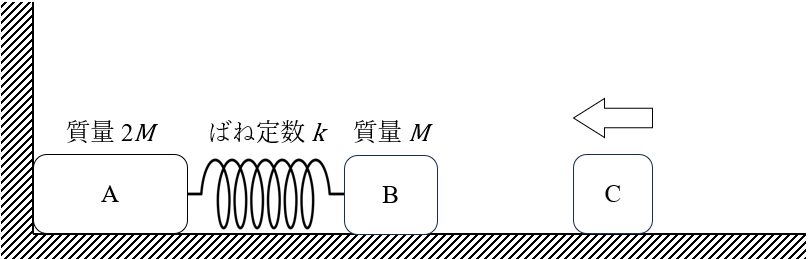
\includegraphics[width=.8\columnwidth]{../graphs/todai_03-1.png}
  \caption{}
\end{figure}


% メモ
\begin{comment}

\end{comment}


%%%%%%%%%%%%%%%%%%
